\documentclass[10pt,a4paper]{article}
\usepackage[T1]{fontenc}
\usepackage[scaled]{helvet}
\usepackage{cite}
\usepackage{url}
\usepackage{graphicx}
\usepackage{float}
\usepackage{amsmath}
\usepackage{amssymb}
\usepackage{fancyhdr}
\usepackage{lastpage}
\floatstyle{boxed} 
\restylefloat{figure}
\renewcommand*\familydefault{\sfdefault}
\title{Digital Computers and Number Systems}
\author{David Lynch}
\begin{document}
\maketitle
\begin{abstract}
This article serves as a gentle introduction to digital computers. Some of you may have covered a lot of this territory already, but it's worth revisiting to illustrate the bare essentials. We will dig in further to some of the topics that are covered here, in particular the areas of memory management and the execution of programs, but for now we will treat the digital computer system at a fairly high level of detail. 
\end{abstract}
\section{Digital Computers}
\subsection{Definition}
At it's most fundamental level, a digital computer facilitates the execution of a sequence of manipulations on inputs, typically, though not always, producing outputs. Physically, the most discreet element of data is a physical quantity called a {\bf signal}. Digital systems will use two discreet values, namely 1 and 0. More often, signals are referred to {\bf bits}. All data in a computer system can be represented as some structured collection of bits. 
\subsection{The Von Neumann Architecture}
John Von Neumann is credited with a laying the groundwork for modern digital computer systems design. Identifiable remnants of his classification of computers into logical units still permeate modern computer systems architectures. In his configuration, computers were apportioned into {\bf memory, central-processing unit and input/output}. Each of these sub-systems is connected by a series of connections known as a {\bf bus}. In the simple design there are three types of bus. The {\bf control bus} is responsible for the transmission of {\bf command data} between the CPU, memory and I/O. Functions such as chip selection, initialization and other forms of control are conducted on this bus. The {\bf data bus} is responsible for the transfer of data between logical units. A separate bus known as the {\bf address bus} is responsible for determining locations for the transfer of data over the data-bus. 

\begin{figure}
\caption{The Von Neumann Architecture \cite{IMGVON}}
\begin{center}
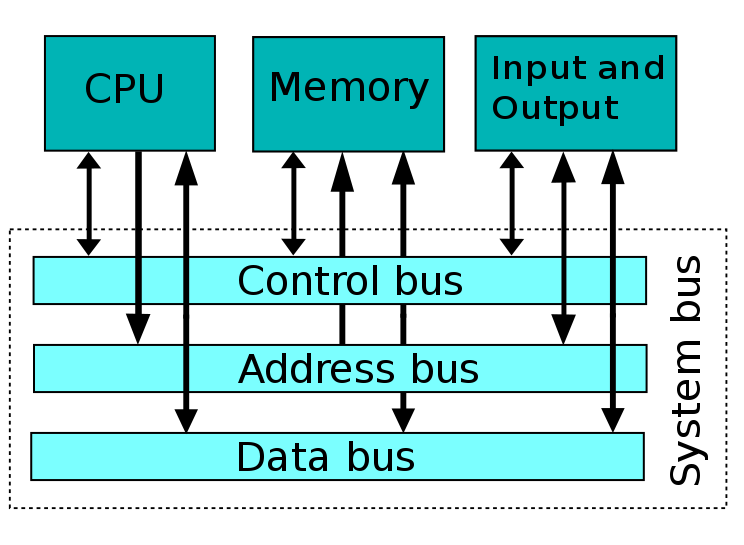
\includegraphics[scale=0.35]{../images/von-neumann.png}
\end{center}
\end{figure}

The following example illustrates how a simple Von-Neumann computer may execute a simple memory write. 
\begin{itemize}
	\item The CPU produces a data output that needs to be stored to memory. 
	\item The CPU will activate the memory component by means of the control bus. 
	\item The CPU will place target memory location on the address bus. 
	\item The CPU will place the data to be written on the data bus. 
\end{itemize} 
\subsubsection{Central Processing Unit}
Commonly known as the CPU, this is the core of the system. The CPU is responsible for the loading and execution of programs, the retrieval and storage of data as well as interaction with external devices. There are two further subdivisions of the CPU which we will consider here. The data path is responsible for the processing of input data and the generation of output data. This includes arithmetic processing (e.g. addition, multiplication) and logical transform (e.g. logical AND, shifting). The {\bf control path} (or unit) is the part of the CPU responsible for supervision and control of data flow between all units in the system. This includes transfer and write-back to memory and provision of inputs and retrieval of outputs from the data path. 
\newline
\newline
The Central Processing Unit can be further divided into units of logical responsibility. In particular, the ALU or Arithmetical and Logical Unit is responsible for the application of fixed precision integer arithmetic and logical operations to the data path. The MMU, or Memory Management Unit is responsible for the management of memory, including memory interaction. In doing so, the MMU provides the CPU with a unified virtual address space. This abstraction allows the CPU to address multiple components, and provides mechanisms for the efficient interaction with these devices.  Lastly, the FPU, or floating point unit is responsible for the execution of floating precision arithmetic. The FPU is a complex unit, which has its own control unit and data path. 
\subsubsection{Memory}
Storage of data is facilitated by memory. There are various forms, differing in characteristics such as {\it durability, access time and capacity} but in general, Memory is a section of the computer where we can store collections of bits. In terms of the Von Neumann architecture, we refer to Main Memory. In computer systems, this is typically RAM or Random Access Memory. More on this later. 
\subsubsection{I/O Devices}
Input and output devices are concerned about how data moves between logical layers external to the CPU and Main Memory. This could mean interaction with an end user by means of a keyboard, or loading of a file into main memory from DVD-ROM or Hard Disk, or even downloading data from the internet via a Network Interface Card (NIC).
\subsubsection{Ancillary Units}
Not really I/O devices and not really a Unit of the Von Neumann architecture, and often digital computers in themselves, ancillary units are an emerging class of component that support the wider computer system by taking responsibility for some specialist function. The primary example is a Graphics Processing Unit (GPU), which in most modern systems is responsible for the efficient provision of computer graphics. Units such as the GPU may directly interact with I/O sub-systems and memory, as well as use specialist data paths custom built for function. In our GPU example, the CPU is typically freed from expensive and constant vector-arithmetic calculations, allowing it to focus on the more general tasks of program control, management and execution. Another example is Cache Memory, which aims to reduce the amount of time a CPU must wait on data to be transferred from Main Memory or an I/O Device.
\newline
\newline
The emergence of ancillary units were at least partially driven to overcome an inefficiency known as {\bf Von-Neumann Bottleneck}. In the illustrated configuration above, the CPU constantly has to read program from memory, while also executing transforms on data. As a result the CPU is quite often waiting around for data to be transferred from memory. This limits the maximum throughput of the CPU. 

\section{Number Systems}
Your maths lecturer will cover number systems in much more detail. Here, I am to introduce the concepts that I will be taken as given for the remainder of the course. When programming computer systems, and understanding of how arithmetic is conducted in digital computers is imperative. What is covered here is the absolute minimum you will need to know to properly tackle some programming problems we will look at later.  
\subsection{Decimal Number System}
All of you are familiar with decimal number systems from primary school. More formally put than counting with your fingers, the decimal number system is represented by strings of digits that are raised to a power of 10 relative to their position in the sequence. The common decimal number system is therefore of {\bf base} or {\bf radix} 10. Each element of the sequence is known as a {\bf coefficient.} 

\begin{center}
$C_{n} C_{n-1} C_{n-2}...C_{1} C_{0}.C_{-1} C_{-2}...C_{-m+1} C_{-m}$
\end{center}
Represents a number system where $n \in \mathbb{I}_{\geq0}, m \in \mathbb{I}_{\geq1}$ and $C \in A$ where $A$ represents the set of possible coefficients in the number system. For the decimal number system $C \in A$ where $A = \{0,1,2,3,4,5,6,7,8,9\}$
\newline\newline
The {\it radix point} - in this case the decimal point - demarcates the transition from positive to negative powers. For example the decimal number 956.75 is expanded as 
$9\times10^2 + 5\times10^1 + 6\times10^0 + 7\times10-^1 + 5\times10-^2$
\newline\newline
The digits at positions $n$ and $m$ in the sequence are known as the {\bf most significant} and {\bf least significant} digits respectively. 
\subsection{Power-of-2 Based Systems}
In the previous section, we discussed the most fundamental element of computer data, the signal. Since a signal can be in one of two states - on, or off - number systems with bases that are powers of two prove to be quite useful. The {\bf binary} number system is the most fundamental of these, with a set of coefficients $A = \{0,1\}$. The restricted size of the coefficient set actually makes binary strings intolerably long for significant cases in which humans must read them. The {\bf octal} - $A= \{[0 - 7]\}$ - and {\bf hexadecimal} - $A = \{[0-9][A-F]\}$ - number systems assist us here. The following shows the decimal number 31 represented in all three number systems. 
\begin{center}
$(31)_{10} = (1F)_{16} = (37)_8 = (11111)_2$
\end{center} 
In understanding capacity to store bits, various methods of grouping size of the sequence together have been devised. One strategy is to raise the number of bits to a factor of 10. In doing this we become familiar with the terms Kilo-, Mega- and Giga-bits which are $2^{10} 2^{20}$ and $2^{30}$ bits respectively.  Another strategy is to group into {\bf bytes} - 8 bits - {\bf words} - 16-bits - or {\bf long words} - 32-bits. These two strategies can also be combined. For example, 1 kilo-byte is 1024 bytes or 1048576 bits. These terms are frequently uses when referring to the capacity of a computer system to store items in memory. 
\subsection{Ranges}
The range of numbers that are representable by a sequence depend on the size of hardware structures that underly. These structures have fixed sizes which are powers of 2. There are various ways to represent numbers which are stored as sequences of bits. An 8-bit word can represent 255 possible integer values including zero. If the integer is unsigned, it is greater than or equal to zero. In this instance the 8-bit word can represent a maximum of 255 and a minimum of zero. We can also use an 8-bits to store signed integer values. This is done typically in one of two ways. In the two's compliment representation, we can store numbers -127 to 128. To calculate the two's compliment, or negative representation, we take the positive value, invert the bits and add 1. In this encoding -2 is represented by the binary string 11111110. Another approach to negative integer representation is a parity bit. In this representation -2 would be represented as 10000010. The disadvatage of this approach is that we have positive and negative representations of zero, allowing us to represent 254 integers.
\newline\newline
The same principle applies to integers represented by 16, 32 or 64 bits. In general the range of numbers representable can be calculated as $0$ to $2^{n} -1$ for unsigned and $-2^{n}/2 + 2$ to $-2^{n}/2 + 1$ for twos compliment unsigned integers where $n$ is the binary string size.    
\subsection{Conversion}
Arithmetic rules follow the same basic concepts for all number systems. To convert to a number system with radix $r$, simply divide by the radix and accumulate the remainders from the least to the most significant bits. 
\begin{table}
\centering
\begin{tabular}{ l c r }
  Addition    & $(58F)_{16} + (E46)_{16}$ & $= (13E5)_{16}$ \\
  Subtraction & $(0101)_2 -(0010)_2$ & $= (011)_2$ \\
\end{tabular}
\caption{Simple arithmetic calculations}
\end{table}
\begin{table}
\centering
\begin{tabular}{ l c r }
  $(156)_{10} / 2$ & $=0$ \\
  $(78)_{10} / 2$ & $=0$  \\
  $(39)_{10} / 2$ & $=1$  \\  
  $(19)_{10} / 2$ & $=1$  \\  
  $(9)_{10} / 2$ & $=1$ \\  
  $(4)_{10} / 2$ & $=0$ \\  
  $(2)_{10} / 2$ & $=0$ \\  
  $(1)_{10} / 2$ & $=1$ \\
\end{tabular}
\caption{$156_{10}$ converted to $10011100_{2}$}
\end{table}
\subsection{Encoding}
The representation of numbers, letters and other data is facilitated by means of encoding. Binary encodings symbolise the underlying numbers that may represent particular characters. A common encoding is ASCII, which uses 7-bit words to encode characters. In this encoding, each character requires a maximum of one byte of space to represent. The ASCII word structure represents addresses in the ASCII table. The format $[ccc][rrrr]$ is used to look-up the table, with the most significant 3 bits of the 7 representing the column lookup and the final 4 bits representing the row. Figure {\ref{ascii}} shows the full ASCII table. 
\begin{figure}
\caption{The ASCII Table\cite{LOGICDESIGN}}
\begin{center}
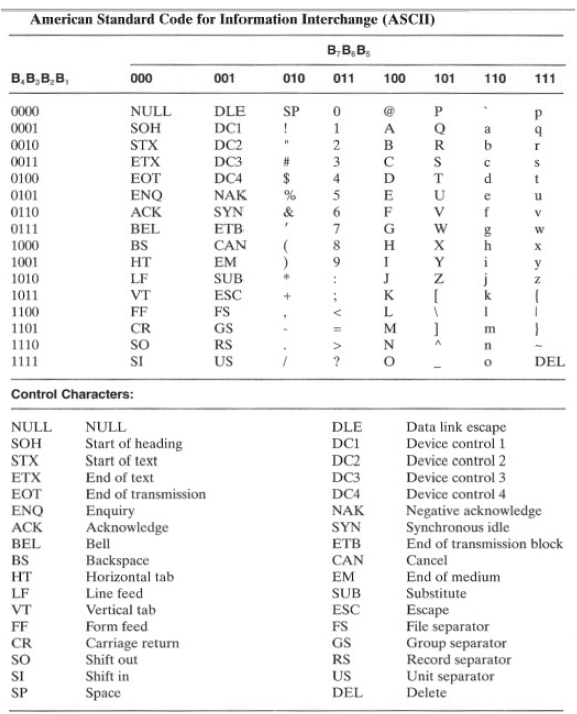
\includegraphics[scale=0.60]{../images/ascii.png}
\label{ascii}
\end{center}
\end{figure}
\bibliography{../biblio/techfundamentals.bib}{}
\bibliographystyle{plain}
\begin{center}
{\small \copyright  David Lynch 2012. Do not reproduce with written permission.}
\end{center}
\end{document}